\subsection{Interpolation - Chapter 18}

\begin{enumerate}

\item {\bf Linear Interpolation}

The simplest form of interpolation is by creating a line in between
points $x_1$ and $x_0$ such that

\begin{equation}
y^* = f(x^*) = f(x_0) + \frac{f(x_1)-f(x_0)}{x_1-x_0}(x^*-x_0)
\end{equation}

\begin{figure}[H]
  \begin{center}
    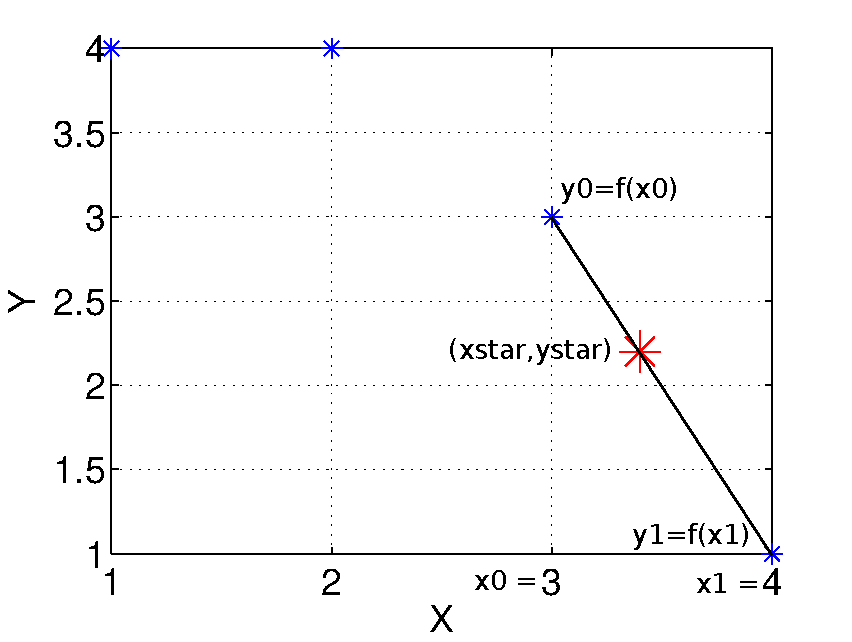
\includegraphics[height=0.5\textwidth,width=0.7\textwidth]{Graphics/Linear_Interpolation.pdf}
  \end{center}
\end{figure}

\item {\bf Polynomial Interpolation}

Note that the problem can be explicitly derived using Linear Regression. That
is we are trying to solve the problem $f(x) = a_0 + a_1(x-x_0)$. If
this problem is set up the solution would yield
$a_0=f(x_0)$ and $a_1$ = {\it slope}. Thus it is possible to extend
the interpolation method to higher order polynomials. Our polynomial
is then

\begin{equation}
\tilde{f}(x) = a_0 + a_1 (x-x_0) + a_2 (x-x_0)^2 + ... a_N (x-x_0)^N
\end{equation}

Note however that in order to interpolate using the equation
above your need N+1 data points. For example, in order to fit a line
the method requires two points to solve for $a_0,a_1$. In order to fit
a quadratic the method requires three points to solve for $a_0,a_1$
and $a_2$.

\begin{figure}[H]
  \begin{center}
    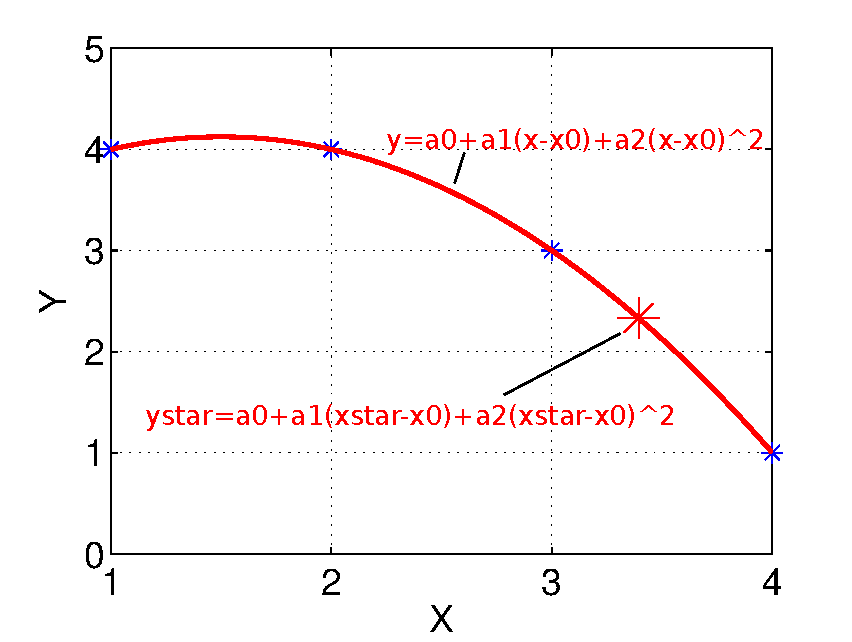
\includegraphics[height=0.5\textwidth,width=0.7\textwidth]{Graphics/Polynomial_Interpolation.pdf}
  \end{center}
\end{figure}

\item {\bf Linear Splines}

Splines are a way to approximate the curve with more than one
model. For example, if you have a curve that looks fourth order you
could fit the entire data set as fourth order polynomial or you could
simply fit the line to 4 linear polynomials. In certain situations
this would actually create a better fit. The equation for linear
splines is simply

\begin{equation}
  \tilde{f}(x) = f(x_{i-1}) + m_{i-1}(x-x_{i-1})~~x_{i-1}\leq x \leq x_i
\end{equation}
where
\begin{equation}
  m_{i-1} = \frac{f(x_{i}) - f(x_{i-1})}{x_{i}-x_{i-1}}
\end{equation}

\item {\bf Quadratic Splines}

The equation for quadratic splines gets a little more messy so the
derivation is left for the student. Instead rules are listed to help
you with the derivation. The basic formula of a quadratic spline is
\begin{equation}
\tilde{f}(x) = a_{i} x^2 + b_{i} x + c_i~~x_{i-1}\leq x \leq x_i
\end{equation}
The rules for quadratic splines are then
\begin{enumerate}
\item The function values of adjacent splines must be equal to each
  other
  \begin{equation}
    a_i x_{i}^2 + b_i x_{i} + c_i = a_{i+1} x_{i}^2 + b_{i+1} x_i + c_{i+1}
  \end{equation}
\item The first and last function must pass through the end points
  \begin{equation}
    \begin{matrix}
      a_1 x_0^2 + b_1 x_0 + c_1 = f(x_0) \\
      a_n x_n^2 + b_n x_n + c_n = f(x_n)
    \end{matrix}
  \end{equation}
\item The first derivative of adjacent splines must be equal to each
  other
  \begin{equation}
    2 a_i x_{i} + b_i = 2 a_{i+1} x_{i} + b_{i+1}
  \end{equation}
\item The second derivative of the first spline at $x_0 = 0$ 
  \begin{equation}
    a_1 = 0
  \end{equation}

\begin{figure}[H]
  \begin{center}
    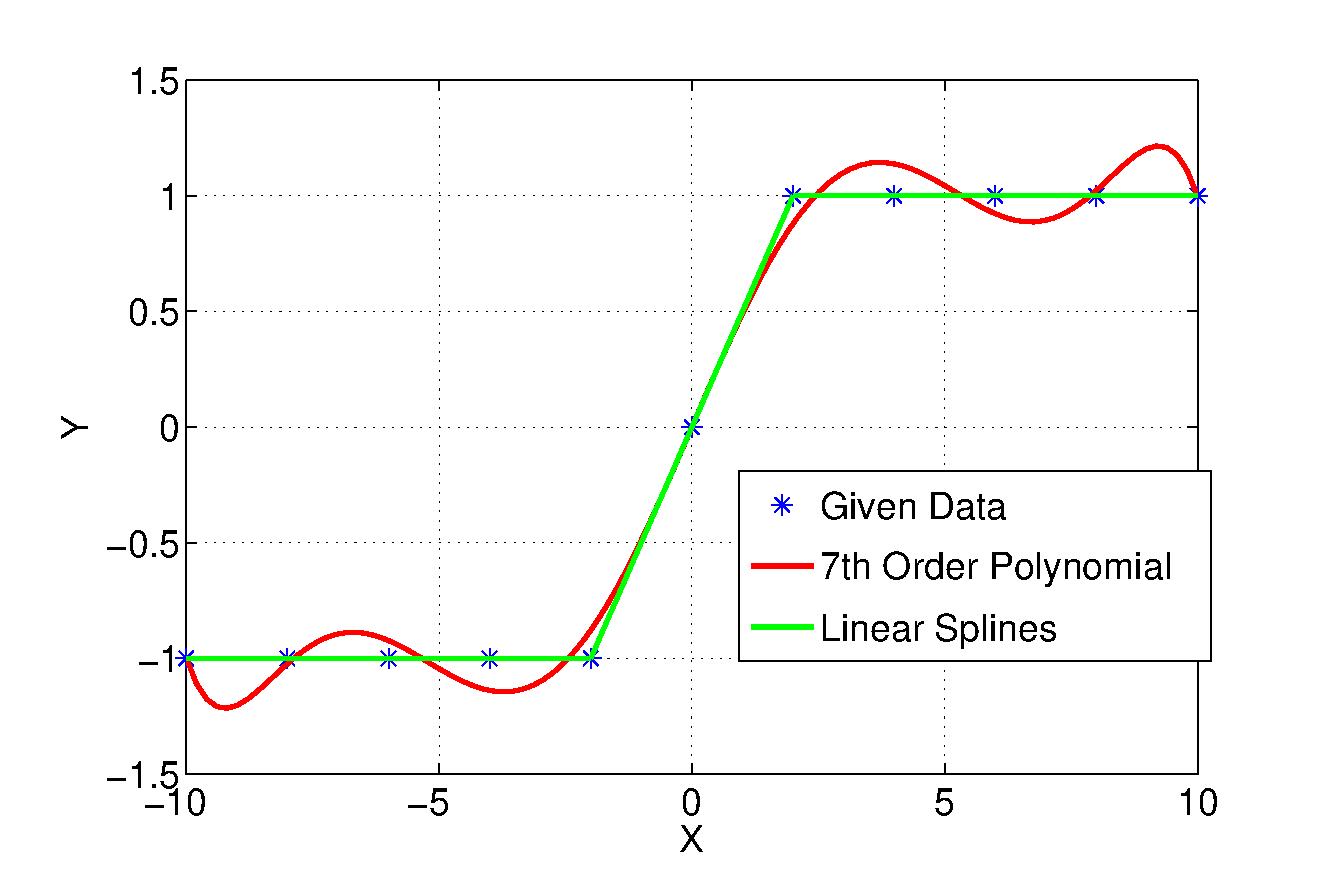
\includegraphics[height=0.5\textwidth,width=0.7\textwidth]{Graphics/Linear_Splines.eps}
  \end{center}
\end{figure}

\clearpage

\begin{figure}[H]
  \begin{center}
    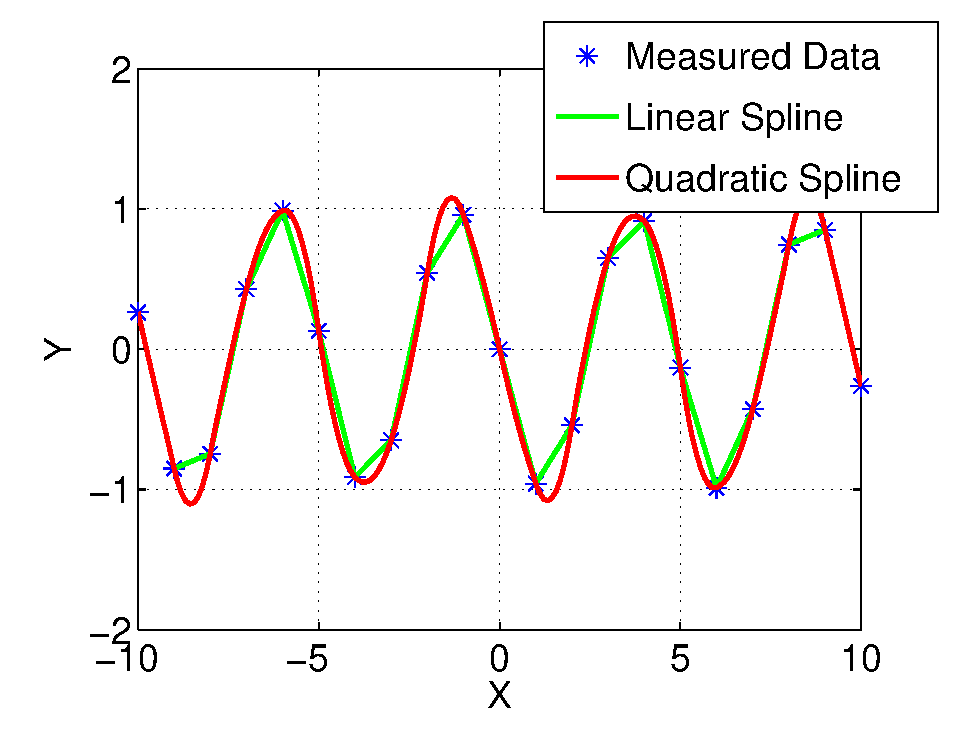
\includegraphics[height=0.5\textwidth,width=0.7\textwidth]{Graphics/Quadratic_Splines.eps}
  \end{center}
\end{figure}

\end{enumerate}

\item {\bf 2-D Interpolation}

It is often the case that rather than your system being of the form
$y=f(x)$ you have an equation of the form $z=f(x,y)$. In this case you
need to use 2-D interpolation and here we will discuss linear 2-D
interpolation called bi-linear interpolation for short. This
interpolation scheme is three separate interpolations. Assume you are
trying to interpolate $z^*=\tilde{f}(x^*,y^*)$ where $x_{i-1}\leq x^*
\leq x_i$ and $y_{i-1}\leq y^* \leq y_i$. The equations to solve for
$z^*$ is then

\begin{equation}
z_U = f(x_{i-1},y_{i}) + \frac{f(x_i,y_i)-f(x_{i-1},y_i)}{x_{i}-x_{i-1}}(x^*-x_{i-1})
\end{equation}
\begin{equation}
z_L = f(x_{i-1},y_{i-1}) + \frac{f(x_i,y_{i-1})-f(x_{i-1},y_{i-1})}{x_{i}-x_{i-1}}(x^*-x_{i-1})
\end{equation}
\begin{equation}
z^* = z_L + \frac{z_U-z_L}{y_i-y_{i-1}}(y^*-y_{i-1})
\end{equation}

The basic solution is simply three linear interpolations to get your
solution.

\begin{figure}[H]
  \begin{center}
    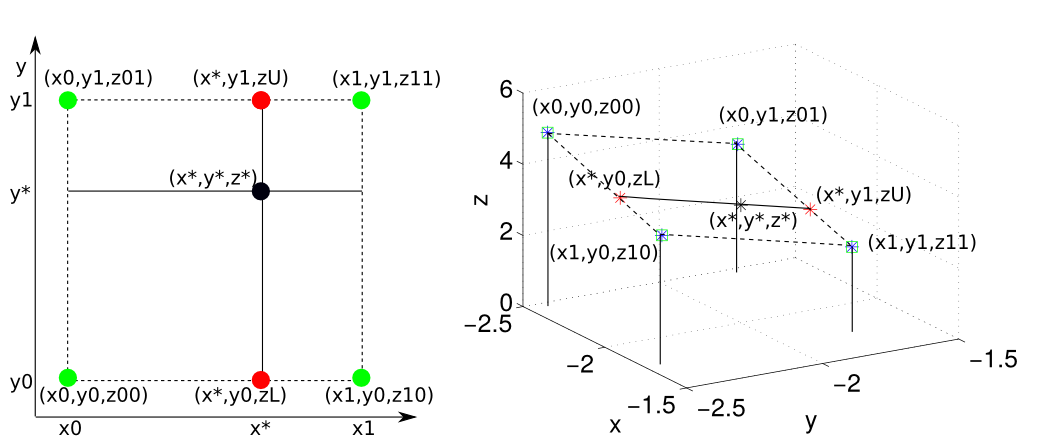
\includegraphics[height=0.4\textwidth,width=0.9\textwidth]{Graphics/TwoD_Interpolation.png}
  \end{center}
\end{figure}

\end{enumerate}
